\documentclass[letterpaper, 11pt]{article}
\usepackage{cite,enumitem,listings, comment}
\usepackage[export]{adjustbox}
\usepackage{amsmath,amssymb,amsfonts}
\usepackage{algorithmic}
\usepackage{graphicx}
\usepackage{textcomp}
\usepackage{graphicx}
\usepackage{geometry}
\usepackage{tabularx}
\usepackage{xcolor}
\usepackage{soul}
\usepackage{chngcntr}
\usepackage{url}
\usepackage{hyperref}
\counterwithin{figure}{subsection}

\begin{document}

%%%%%%%%%%%%%%%% Document Starts %%%%%%%%%%%%%%%%%%%%%

% Title page 
\title{Aviator Design Document}
\author{David Thoe, Joshua Kim, Zeke Ulrich, Juan Vargas}
\date{\today}
\maketitle

\begin{center}
    GTA: Zixiao Ma \\
    Professor: Ryan Beasley
\end{center}

% Sketch goes here
\begin{figure}[h]
    \centering
    
\includegraphics[width=12cm,scale=1]{images/white.png}
    \caption{[Caption]}
\end{figure}

\clearpage
\tableofcontents

\clearpage
\listoffigures

\clearpage
\listoftables

% Revision Log Page
\clearpage
\section*{Revision Log}
% For every update, copy a whole LATEX code line and adjust 
% accordingly. In theory, update every time you make major 
% changes in the document. The \& symbol serves to separate 
% items in the table. If you are new to this, align the \& 
% so that it looks more like a table in the code. 
\begin{table}[h]
    \begin{tabularx}{\textwidth}{|l|c|X|} % 
        \hline
        Date      & Revision & Changes         \\ \hline
        5/3/2024  & v0.1     & Initial Release \\ \hline
        9/18/2025 & v1.0     & First Draft     \\ \hline
    \end{tabularx}
    \caption{Revision Log}
\end{table}

% Glossary Page
\clearpage
\section*{Glossary} % Document key words and acronyms here. 
\begin{itemize}
    \item \textbf{API} Application Programming Interface.
\end{itemize}

\clearpage
\section{Introduction}
\subsection{Executive Description}

Retro nearby flight information display.

\subsection{User Stories}

\paragraph{User Story 1 – The Long-Time Aviation Hobbyist\newline} 
	As a long-time aviation hobbyist who has spent years tracking flights through phone apps, I’m tired of paying for subscriptions just to unlock basic features. 
    I want a device that gives me real-time flight information without hidden costs, while also providing a tactile, nostalgic experience that reminds me of classic aviation boards. 
    By having the Aviator on my desk, I can finally stay connected to the aviation world without feeling like I’m paying a premium for something that should be standard and accessible.   

\paragraph{User Story 2 – The Casual Aviation Enthusiast\newline} 
	As someone with a general interest in aviation, I don’t need a full cockpit-level tracker, but I do want something that feels engaging and easy to use. 
    Standard apps are flat, cluttered, and frankly too much for a novice like myself, but the Aviator project makes flight tracking simple, physical, and fun. 
    I can glance at the board, see arrivals and departures, and feel connected to the aviation scene effortlessly. The setup process was simply plug and play. 
    Additionally, I don’t have to pay a dime for the product. For me, it’s about accessibility and enjoying aviation in a personal,low-effort, high-impact way.

\paragraph{User Story 3 – The Purdue ECE Student\newline}
	As a Purdue ECE student, I’m drawn to the Aviator not only as a hobby project that I can tinker with, but also as a nod to Purdue’s deep aviation legacy. 
    It’s inspiring to own a piece of tech that bridges my academic interests in circuits and embedded systems with Purdue’s reputation in aerospace. 
    I want a tracker that feels hands-on, customizable, and personal—something that makes me feel part of both my field of study and Purdue’s aviation history every time I glance at it. 
    Given the nature of the project and its ability to be completed by an individual excites me, as it gives me the stepping stone I needed to start tracking flights.

\clearpage
\section{Design Requirements}
\subsection{Requirements}
\begin{enumerate}
    \item {[Type here \textbf{DD1+}]}
    \item {[Type here \textbf{DD1+}]}
\end{enumerate}

\clearpage

\subsection{Factors Influencing Requirements}
\subsubsection{Public Health, Safety, and Welfare}
\begin{enumerate}
    \item The display must not interfere with
          user's well-being by, for example, displaying at
          excessive luminosity or updating rapidly
          in a distracting manner.
    \item The device must not infringe on any person's
          reasonable expectation of privacy.
\end{enumerate}

\subsubsection{Cultural Factors}
\begin{enumerate}
    \item The device must
          be language-agnostic wherever possible.
    \item The design must be culturally neutral
          cannot presuppose exposure to similar
          technology.
\end{enumerate}

\subsubsection{Social Factors}
\begin{enumerate}
    \item The physical device should be
          easily replicated with widely available
          parts.
    \item The code for the device must
          be open-source and well-documented.
\end{enumerate}

\subsubsection{Environmental Factors}
\begin{enumerate}
    \item The device should be as durable and
          environmentally friendly as possible so as
          not to contribute to e-waste.
    \item The device must not contribute to noise
          or visual pollution of any space.
    \item The device must be energy-efficient.
\end{enumerate}

\subsubsection{Economic Factors}
\begin{enumerate}
    \item The device must minimize
          construction and recurring costs.
    \item The device must not infringe on
          right to repair.
\end{enumerate}
\clearpage
\section{System Overview}
\subsection{System Block Diagram}
\begin{figure}[h]
    \centering
    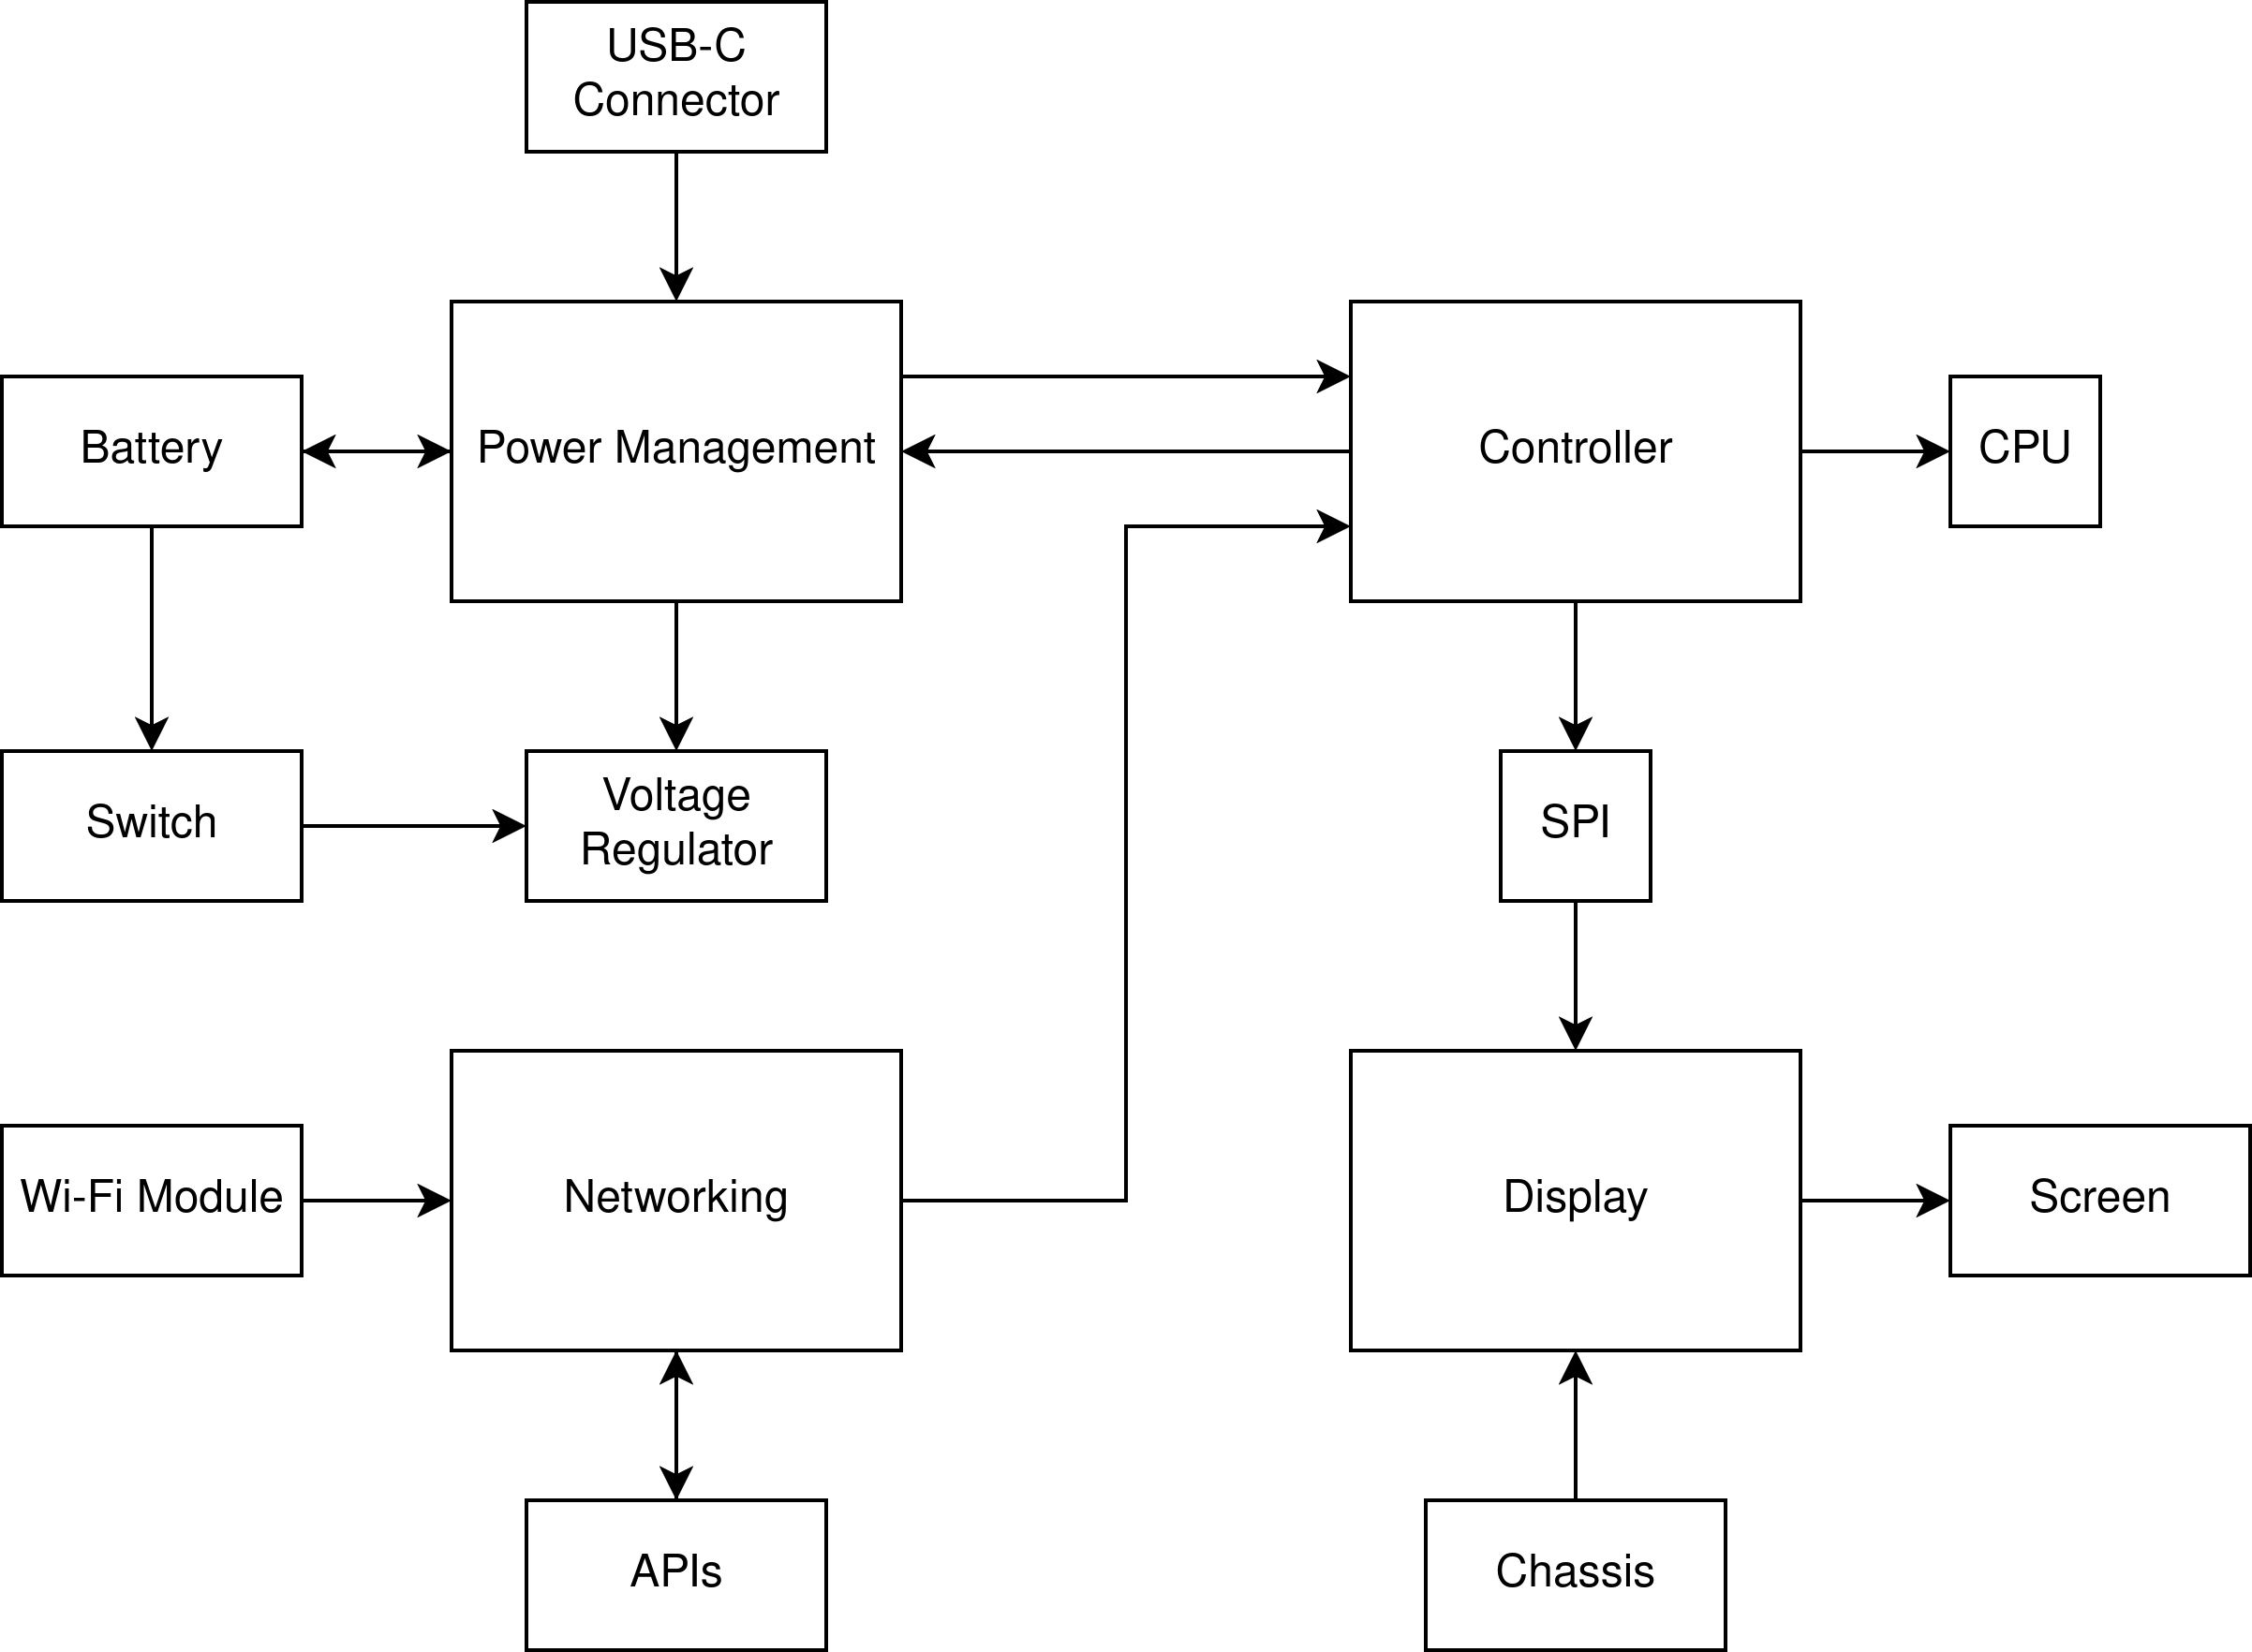
\includegraphics[width=16cm]{images/block_diagram.png}
    \caption{System Block Diagram}
\end{figure}

% Activity Diagram
\clearpage
\subsection{System Activity Diagram}
[\textbf{DD1+}]
\begin{figure}[h]
    \centering
    
\includegraphics[width=16cm]{images/white.png} % Change the picture
    \caption{System Activity Diagram}
\end{figure}

% Mechanical Design
\clearpage
\subsection{System Mechanical Design (Extra Credit)}
[\textbf{DD3+}]
\begin{figure}[h]
    \centering
    
\includegraphics[width=16cm]{images/white.png} % Change the picture
    \caption{System Mechanical Design}
\end{figure}

% Integration Approach
\clearpage
\subsection{Integration Approach}
[\textbf{DD3+}]
[Theory behind the system design, with reference to subsystem integration within your system – i.e., explain how it is supposed to work, but not whether it did actually work]
[Type here]

% System Photograph
\clearpage
\subsection{System Photographs} % Have as many photoes as you need
[\textbf{DD3+}]
[Photograph of assembled system, intended to highlight user interaction / controls. If system is split into multiple parts, show a composite of more than one photograph with all key user interactions / controls. ]
\begin{figure}[h]
    \centering
    
\includegraphics[width=16cm]{images/white.png} % Change the picture
    \caption{[Photo Name]}
\end{figure}
\section{Subsystems}
%%%%%%%%%%%%% Subsystem 1 %%%%%%%%%%%%%%%
\subsection{Subsystem 1: [Subsystem Name]}

% Subsystem Diagram
\subsubsection{Subsystem Diagrams}
[\textbf{DD1+}]
\begin{figure}[h]
    \centering
    
\includegraphics[width=16cm]{images/white.png} % Change the picture
    \caption{Subsystem Block Diagram}
\end{figure} % If your subsystem is more coding, change it to activity diagram

% Specifications
\subsubsection{Specifications}
\begin{enumerate}
    \item {[Type here \textbf{DD1+}]}
\end{enumerate}

% Subsystem Interactions
\subsubsection{Subsystem Interactions}
[Type here \textbf{DD1+}]

% Core ECE
\subsubsection{Core ECE Design Tasks}
[\textbf{DD1+} Write tasks and course that helps accomplish that task]
\begin{itemize}
    \item \textbf{ECE xxxxx}: [Type the relationship here. ]
\end{itemize}

% Schematics
\subsubsection{Schematics}
[Type here \textbf{DD2+}]
\begin{figure}[h]
    \centering
    
\includegraphics[width=16cm]{images/white.png} % Change the picture
    \caption{[Schematic Name]}
\end{figure} % If your subsystem is more coding, change it to psudo code

% Parts List
\subsubsection{Parts}
\begin{itemize}
    \item {[Type here \textbf{DD1+}]}
\end{itemize}

% Algorithm
\subsubsection{Algorithm}
[Type here \textbf{DD1+}]

% Theory of Operation
\subsubsection{Theory of Operation}
[Type here \textbf{DD2+}]

% Specification Measurement
\subsubsection{Specifications Measurement}
[\textbf{DD3+} Every specification here should match the specification above. ]
\begin{enumerate}
    \item {[Copy specification here. ]} \\
          {[Explain the specification here. Add photoes if necessary. ]}
\end{enumerate}

% Standards
\subsubsection{Standards}
[\textbf{DD1+}]
\begin{itemize}
    \item \textbf{[Standard Name]}: [Describe the standards and explain the connection]
\end{itemize}
\clearpage
\subsection{Subsystem 2: Power Management}

% Subsystem Diagram
\subsubsection{Subsystem Diagrams}
[\textbf{DD1+}]
\begin{figure}[h]
    \centering
    
\includegraphics[width=16cm]{images/white.png} % Change the picture
    \caption{Subsystem Block Diagram}
\end{figure} % If your subsystem is more coding, change it to activity diagram

% Specifications
\subsubsection{Specifications}
\begin{enumerate}
    \item {[Type here \textbf{DD1+}]}
\end{enumerate}

% Subsystem Interactions
\subsubsection{Subsystem Interactions}
[Type here \textbf{DD1+}]

% Core ECE
\subsubsection{Core ECE Design Tasks}
[\textbf{DD1+} Write tasks and course that helps accomplish that task]
\begin{itemize}
    \item \textbf{ECE xxxxx}: [Type the relationship here. ]
\end{itemize}

% Schematics
\subsubsection{Schematics}
[Type here \textbf{DD2+}]
\begin{figure}[h]
    \centering
    
\includegraphics[width=16cm]{images/white.png} % Change the picture
    \caption{[Schematic Name]}
\end{figure} % If your subsystem is more coding, change it to psudo code

% Parts List
\subsubsection{Parts}
\begin{itemize}
    \item USB-C 5 V input module
    \item Li-ion battery pack (3.7 V, 8000 mAh)
    \item Buck-boost regulator IC (for 3.3 V and 5 V rails)
    \item Battery charging IC (USB-C PD or simple Li-ion charger).
    \item Basic protection devices (fuse, MOSFET switch, TVS diode).
    \item (Optional) Solar panel (5–20 W) + MPPT controller IC.
\end{itemize}

% Algorithm
\subsubsection{Algorithm}
[Type here \textbf{DD1+}]

% Theory of Operation
\subsubsection{Theory of Operation}
[Type here \textbf{DD2+}]
% Specification Measurement
\subsubsection{Specifications Measurement}
[\textbf{DD3+} Every specification here should match the specification above. ]
\begin{enumerate}
    \item {[Copy specification here. ]} \\
          {[Explain the specification here. Add photoes if necessary. ]}
\end{enumerate}

% Standards
\subsubsection{Standards}
[\textbf{DD1+}]
\begin{itemize}
    \item \textbf{USB-C Power Delivery Specification}: ensures safe and standard input power.
    \item \textbf{IEEE 1625}: covers battery system reliability for portable electronics.
    \item \textbf{UL 2054}: safety standard for rechargeable batteries in consumer devices.
    \item \textbf{IEC 61215}: (Optional solar) performance and reliability for PV modules.
\end{itemize}

\subsection{Subsystem 3: Text Display \& Chassis}

% Subsystem Diagram
\subsubsection{Subsystem Diagrams}
\begin{figure}[h]
    \centering
    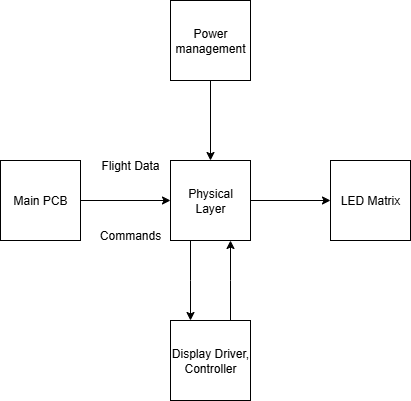
\includegraphics[width=12cm]{images/blockDiagram-display.png} % Change the picture
    \caption{Subsystem Block Diagram}
\end{figure} % If your subsystem is more coding, change it to activity diagram

% Specifications
\subsubsection{Specifications}
\begin{enumerate}
    \item Feature a 2056-pixel Dot Display (128 x 256px)
    \item Physical dimensions of housing within 5\% of 64 x 128 x 256 mm.
\end{enumerate}

% Subsystem Interactions
\subsubsection{Subsystem Interactions}
The display subsystem links the main PCB and the LED Matrix. This subsystem will interface with the power management system and the main PCB. It will recieve data and commands from the main PCB, interpret the commands, and display the data.

% Core ECE
\subsubsection{Core ECE Design Tasks}
\begin{itemize}
    \item \textbf{ECE 27000}: Provides a solid foundation in logic circuits. Helps for designing registers, data paths, logic that drives the LED panel.
    \item \textbf{ECE 25500}: Provides a base understanding of transisters, amplifiers, and fundamentals into I-V behavior.
    \item \textbf{ECE 40862}: Teaches valuable STM concepts such as programming, interrupts, and DMA which are needed to drive the display controller efficiently.
\end{itemize}

% Schematics
\subsubsection{Schematics}
[Type here \textbf{DD2+}]
\begin{figure}[h]
    \centering
    
\includegraphics[width=16cm]{images/white.png} % Change the picture
    \caption{[Schematic Name]}
\end{figure} % If your subsystem is more coding, change it to psudo code

% Parts List
\subsubsection{Parts}
\begin{itemize}
    \item {[Type here \textbf{DD1+}]}
    \item 32 x 64 px LED Matrix (ADAFruit from DigiKey)
    \item 
\end{itemize}

% Algorithm
\subsubsection{Algorithm}

\begin{lstlisting}
    Initialize:
    Configure GPIOs for DATA, CLK, LAT, OE, row select lines (A,B,C,D)
    Initialize interface for incoming data
    Initialize timer for refresh interrupts
    Set PWM resolution (e.g., 8-bit)

    Main Loop:
    while (true):
        if new frame data available from main PCB:
            copy frame buffer into local memory (double buffer optional)
        
        for each row_index in 0 .. NUM_ROWS-1:
            select_row(row_index)        
            OE = HIGH                   
            
            for pwm_bit = 7 downto 0:    // for 8-bit PWM
                for col_index = 0 .. NUM_COLS-1:
                    pixel = frame_buffer[row_index][col_index]
                    if pixel.red  & (1 << pwm_bit) != 0:
                        DATA_R = HIGH
                    else:
                        DATA_R = LOW
                    if pixel.green & (1 << pwm_bit) != 0:
                        DATA_G = HIGH
                    else:
                        DATA_G = LOW
                    if pixel.blue & (1 << pwm_bit) != 0:
                        DATA_B = HIGH
                    else:
                        DATA_B = LOW
                    
                    pulse(CLK)           
                    
                pulse(LAT)                
                OE = LOW                   
                delay(PWM_DELAY[pwm_bit])  
                
        repeat indefinitely
\end{lstlisting}

% Theory of Operation
\subsubsection{Theory of Operation}
[Type here \textbf{DD2+}]

% Specification Measurement
\subsubsection{Specifications Measurement}
[\textbf{DD3+} Every specification here should match the specification above. ]
\begin{enumerate}
    \item {[Copy specification here. ]} \\
          {[Explain the specification here. Add photoes if necessary. ]}
\end{enumerate}

% Standards
\subsubsection{Standards}
[\textbf{DD1+}]
\begin{itemize}
    \item \textbf{[Standard Name]}: [Describe the standards and explain the connection]
\end{itemize}
%%%%%%%%%%%%% Subsystem 4 %%%%%%%%%%%%%%%
\clearpage
\subsection{Subsystem 4: Network and Communications}

% Subsystem Diagram
\subsubsection{Subsystem Diagrams}
[\textbf{DD1+}]
\begin{figure}[h]
    \centering
    
\includegraphics[width=16cm]{images/white.png} % Change the picture
    \caption{Subsystem Block Diagram}
\end{figure} % If your subsystem is more coding, change it to activity diagram

% Specifications
\subsubsection{Specifications}
\begin{enumerate}
    \item {[Type here \textbf{DD1+}]}
\end{enumerate}

% Subsystem Interactions
\subsubsection{Subsystem Interactions}
[Type here \textbf{DD1+}]

% Core ECE
\subsubsection{Core ECE Design Tasks}
[\textbf{DD1+} Write tasks and course that helps accomplish that task]
\begin{itemize}
    \item \textbf{ECE xxxxx}: [Type the relationship here. ]
\end{itemize}

% Schematics
\subsubsection{Schematics}
[Type here \textbf{DD2+}]
\begin{figure}[h]
    \centering
    
\includegraphics[width=16cm]{images/white.png} % Change the picture
    \caption{[Schematic Name]}
\end{figure} % If your subsystem is more coding, change it to psudo code

% Parts List
\subsubsection{Parts}
\begin{itemize}
    \item Weather API
    \item Flight API
    \item Time Sync API
    \item GPS/Geolocation API
    \item Network Interface
    \item Data/Signal Interface
\end{itemize}

% Algorithm
\subsubsection{Algorithm}
[Type here \textbf{DD1+}]

% Theory of Operation
\subsubsection{Theory of Operation}
[Type here \textbf{DD2+}]

% Specification Measurement
\subsubsection{Specifications Measurement}
[\textbf{DD3+} Every specification here should match the specification above. ]
\begin{enumerate}
    \item {[Copy specification here. ]} \\
          {[Explain the specification here. Add photos if necessary. ]}
\end{enumerate}

% Standards
\subsubsection{Standards}
\begin{itemize}
    \item \textbf{NMEA 0183}: Used by GPS receivers to format location/time data, ensuring compatibility with processing algorithms.
    \item \textbf{REST/HTTPS}: Secure, standardized communication with weather servers and external data sources.
    \item \textbf{IEEE 802.11 (Wi-Fi) / IEEE 802.3 (Ethernet)}: Provides reliable networking for internet-based data exchange (when we add website interference).
    \item \textbf{TCP/IP, Checksum validation}: Ensures robustness in communication so that even non-technical users get accurate, reliable results.
\end{itemize}
\clearpage
\section{PCB Design}
\subsection{PCB Schematics}
[\textbf{DD3+}]
\begin{figure}[!h]
    \centering
    
\includegraphics[width=10cm]{images/white.png} % Change the picture
    \caption{PCB Schematic}
\end{figure}

\clearpage
\subsection{PCB Layout}
[\textbf{DD3+}]
\begin{figure}[h]
    \centering
    
\includegraphics[width=16cm]{images/white.png} % Change the picture
    \caption{PCB Layout}
\end{figure}
%%%%%%%%%%%%%%% Final Status Page %%%%%%%%%%%%%%%%%%
\clearpage
\section{Final Status of Requirements}
 [\textbf{DD3+}]
 [If met, give a detailed explanation of the requirement. If partially met, mention what has been met and a reason for why the complete requirement couldn’t be achieved. If not met, give an explanation for why the requirement couldn’t be met in the product. Add as many requirements as you had in your earlier design documents here. ]
\begin{enumerate}
    \item Requirement 1: [Copy your requirement above here] \\
          \textbf{Met}: [Explanation]
    \item Requirement 2: [Copy your requirement above here] \\
          \textbf{Partially Met}: [Explanation]
    \item Requirement 3: [Copy your requirement above here] \\
          \textbf{Not Met}: [Explanation]
\end{enumerate}

%%%%%%%%%%%%%%% Team Intro Page %%%%%%%%%%%%%%%%%%%%
\clearpage
\section{Team Structure}
 [\textbf{DD1+}]
\subsection{Team Member 1}

\includegraphics[height=4cm]{images/white.png} \\
\textbf{[Name Here]}\\
Major: [FILL IN]\\
Contact: [user]@purdue.edu\\
Team Role: [Technical and Professional Roles in the team] \\
Bio: [Short Introduction here]

\subsection{Team Member 2}

\includegraphics[height=4cm]{images/white.png} \\
\textbf{[Name Here]}\\
Major: [FILL IN]\\
Contact: [user]@purdue.edu\\
Team Role: [Technical and Professional Roles in the team] \\
Bio: [Short Introduction here]

\subsection{Team Member 3}
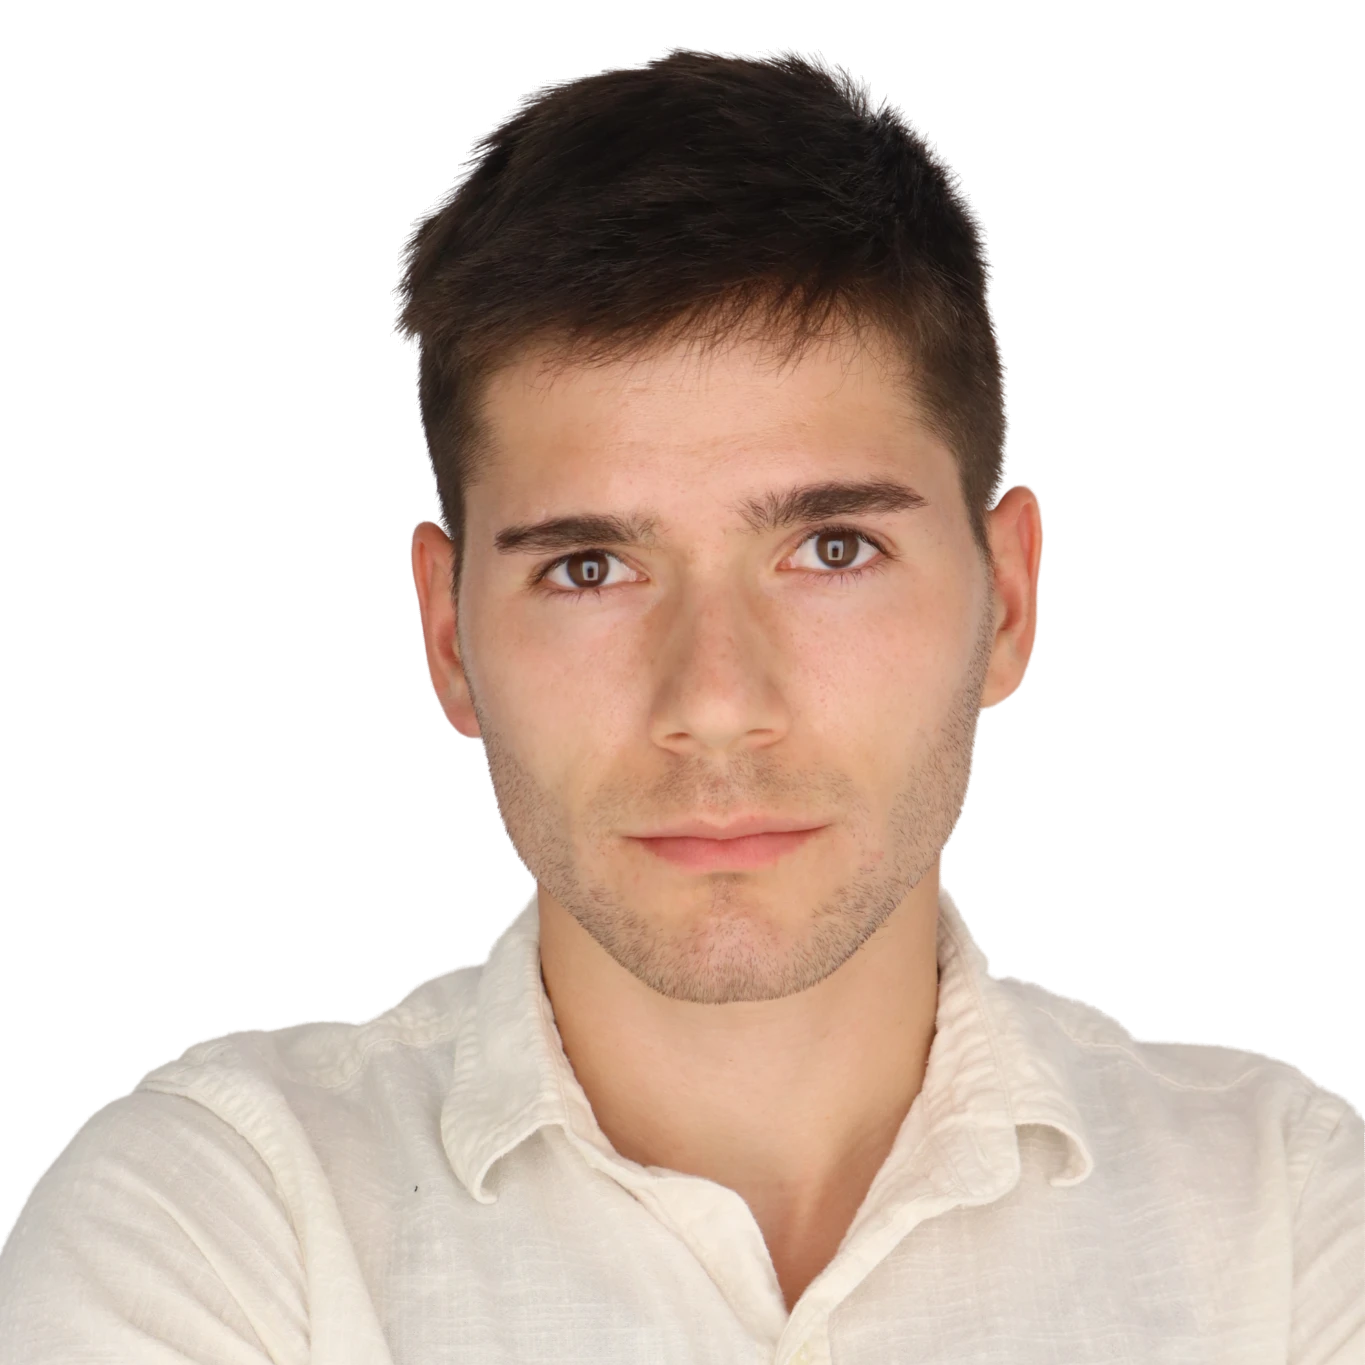
\includegraphics[height=4cm]{images/zeke.png} \\
\textbf{Zeke Ulrich}\\
Major: Computer Engineering\\
Contact: pulrich@purdue.edu\\
Team Role: Treasurer \\
Bio: Zeke is the processing and PCB design specialist.
At Purdue, he belongs to the Marine Corp Officer Candidate Program,
Eta Kappa Nu, Tau Beta Pi, and Purdue's Effective Altruism community.
Outside Purdue, he is president of the nonprofit DuelGood and works
for the government in cybersecurity.
In the future he hopes to study international relations as a Truman
scholar, start a family, and volunteer as a firefighter.
He enjoys athletics and spending time with his friends.

\subsection{Team Member 4}

\includegraphics[height=4cm]{images/white.png} \\
\textbf{[Name Here]}\\
Major: [FILL IN]\\
Contact: [user]@purdue.edu\\
Team Role: [Technical and Professional Roles in the team] \\
Bio: [Short Introduction here]

%%%%%%%%%%%%%%%%% Biblography %%%%%%%%%%%%%%%%%%%%%%%
\clearpage
\section{Bibliography}

 [Here are some examples. IEEE format can be found on \href{https://owl.purdue.edu/owl/research_and_citation/ieee_style/ieee_overview.html}{\hl{Purdue OWL}}. ]

\begin{thebibliography}{}

    \bibitem{b1}
    “Data Platform - Open Power System data,” Apr. 15, 2020. https://data.open-power-system-data.org/household\_data/

    \bibitem{b2}
    Author,"Title," \emph{Journal},volume,number, page range, month year, DOI.

    \bibitem{b3}
    Author. "Page."Website. URL(accessed month day,year)

\end{thebibliography}

%%%%%%%%%%%%%%%%% Appendix %%%%%%%%%%%%%%%%%%%%%%%%%
\clearpage
\section{Appendices}
 [This section is mainly designed for code.
  You can directly generate a somewhat decent display
  of your code file or psuedo code by using the template provided below. You can have as many appendix as you want. In the document, you can refer to the code posted here instead of pasting the whole code in the body. ]

\include{chapters/appendix}

\end{document}
